\subsection{Magnetfelder von stromdurchgeflossenen Leitern}

Oersted (1820): Magnetische Wirkung eines geschlossenen Stromkreises
\break
$ \Rightarrow $ wenn $ I \neq 0 $: Drehmoment auf Kompassnadel, $ \vec{M}=\vec{\mu}\times \vec{B} $ \\
$ \Rightarrow $ $ \vec{B} $ in Ebene $ \perp $ Leiter \\
$ \Rightarrow $ Richtung (Vorzeichen, VZ) ist abhängig von Stromrichtung (Rechtsschraubregel)
\begin{center}
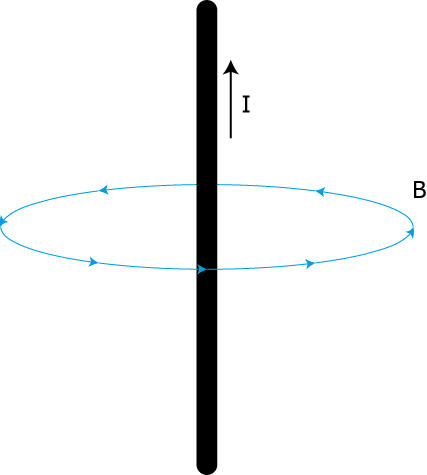
\includegraphics[width=0.4\linewidth]{skizzen/16/16_2B01}
\end{center}

\subsubsection{Bestimmung der Abstandsabhängigkeit}
$$ |\vec{B}| \sim \frac{I}{r}$$
$ \Rightarrow $ Beachte: "Quelle" des Magnetfeldes ist 1D $ \Rightarrow $ Abstandsabhängigkeit \\
quantitativ:
	\begin{align*}
		\boxed{|\vec{B}|=\frac{\mu_0}{2\pi} \cdot \frac{I}{r} }\\
		\mu_0 = \SI{4\pi e-7}{\newton\per\ampere^2} \text{magnetische Konstante}
	\end{align*}
	
\begin{center}
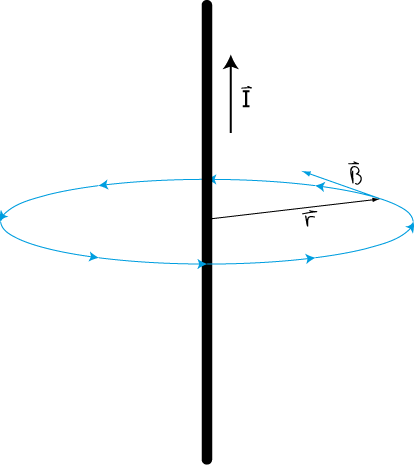
\includegraphics[width=0.4\linewidth]{skizzen/16/16_2B02}
\end{center}


$ \Rightarrow $ Bewegte Ladungen erzeugen ein Magnetfeld in Richtung: $ \frac{\vec{v}}{|\vec{v}|} \times \frac{\vec{r}}{|\vec{r}|}  $ \\
Bisher:
\begin{itemize}
	\item $ \vec{B} $-Feld übt Kraft auf bewegte Ladung aus
	\item Bewegte Ladung (Strom) erzeugt Magnetfeld
\end{itemize}
$ \Rightarrow $ Wechselwirkung zwischen Strömen muss existieren!

\begin{center}
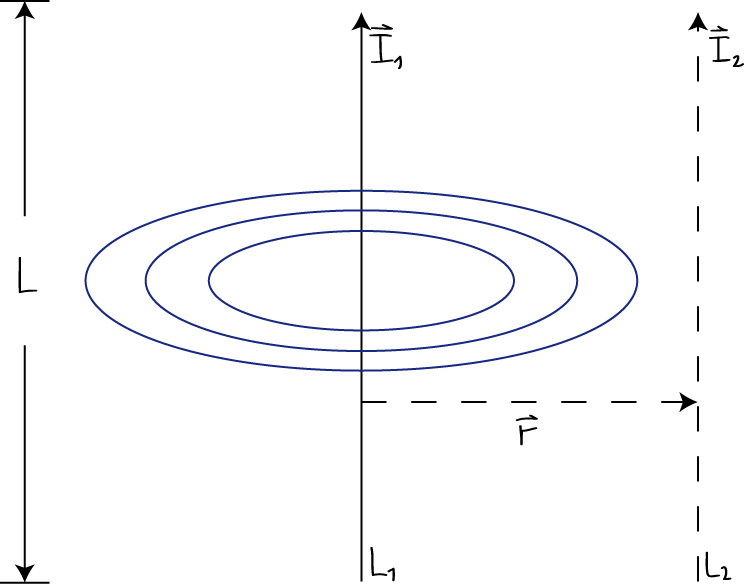
\includegraphics[width=0.4\linewidth]{skizzen/16/16_2B03}
\end{center}


$ I_1 $ erzeugt $ \vec{B} $-Feld am Ort des Leiters $ L_2 $
$$ |\vec{B}_1| = \frac{\mu_0}{2\pi} \cdot \frac{I_1}{r} $$
$ \Rightarrow $ Kraft auf $ L_2 $
\begin{center}
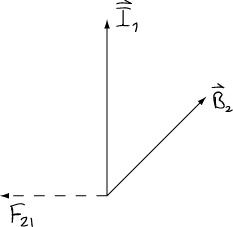
\includegraphics[width=0.2\linewidth]{skizzen/16/16_2B04}
\end{center}

\begin{align*}
\vec{F}_{21} = L \cdot \vec{I}_2 \times \vec{B}_1\\
|\vec{F}_{21}| &= \frac{\mu_0}{2\pi} \cdot \frac{I_1 \cdot I_2}{r} \cdot L\\
&= \underline{\underline{\num{2e-7} \cdot \frac{I_1 \cdot I_2}{r} \cdot L}}
\end{align*}
$ \vec{F}_{21} $: anziehend bei parallelen Strömen! 
\subsubsection{Definition Ampere}
\paragraph{Elektrische Stromstärke: Ampere [A]}
Das Ampere ist die Stärke eines konstanten elektrischen Stromes, der, durch zwei parallele, gradlinige, unendlich lange und im Vakuum im Abstand von einem Meter voneinander angeordnete Leiter von vernachlässigbar kleinem, kreisförmigem Querschnitt fließend, zwischen diesen Leitern je einem Meter Leiterlänge die Kraft $ \SI{2e-7}{\newton} $ hervorrufen würde.\hfill \break

Ströme parallel:\\
\begin{center}
	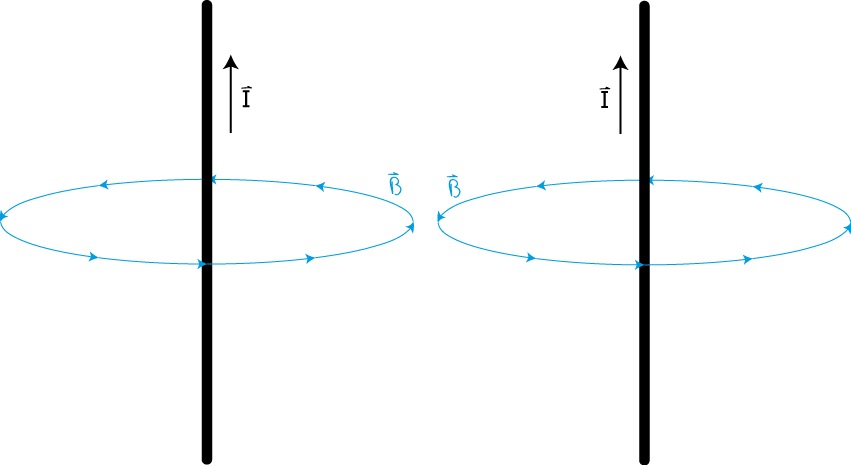
\includegraphics[width=0.4\linewidth]{skizzen/16/16_2B05}
\end{center}
$ I_1 \uparrow\downarrow I_2 $ \\
\begin{center}
	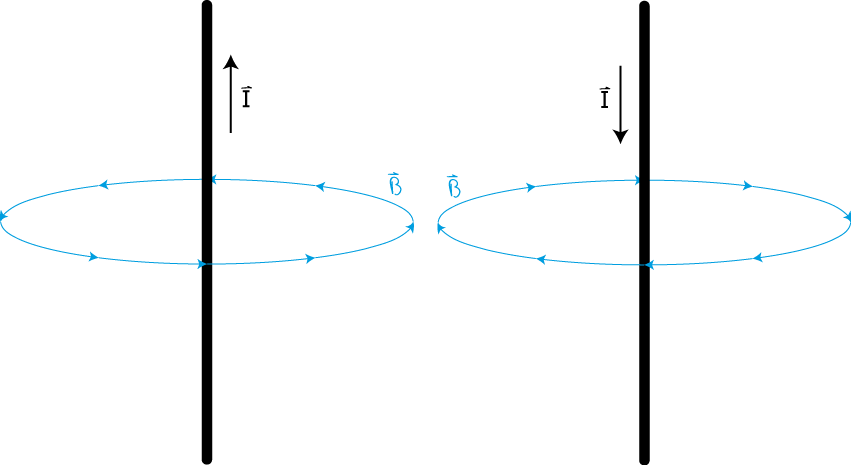
\includegraphics[width=0.4\linewidth]{skizzen/16/16_2B06}
\end{center}

Elektrostatik: Gaußscher Satz: Zusammenhang zwischen Quellen-Verteilung und Feldstärke! \\
\indent $ \Rightarrow $ Normalkomponente des $ \vec{E} $-Feldes wichtig\\
Hier: Ströme als "Quelle" des magnetischen Feldes \\
"Umhüllung" der Ströme \underline{ohne} die Quelle zu "schneiden" nur mit geschlossenem Umlauf möglich (Quellen \underline{nicht} punktförmig!)\\
Beachte also: $ \displaystyle \oint\vec{B}d\vec{s} $
\begin{center}
	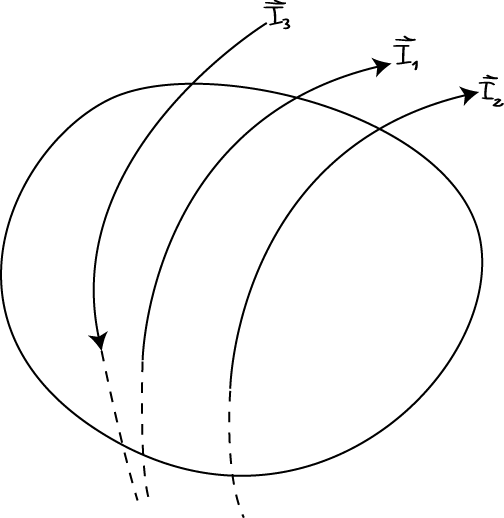
\includegraphics[width=0.4\linewidth]{skizzen/16/16_2B08}
\end{center}
Integrieren über $ dl $ ($ 0...2\pi $) statt über die Länge der Kurve \\
\begin{align*}
\vec{B} \cdot d\vec{s} &= B \cdot r \cdot dl\\
&= \frac{\mu_0}{2\pi} \cdot \frac{I}{r} \cdot dl = \frac{\mu_0}{2\pi} \cdot I \cdot dl \\
\end{align*}
$$ \boxed{{\displaystyle \oint \vec{B}\cdot d\vec{s} = \frac{\mu_0 \cdot I}{2\pi} \oint dl = \mu_0 \cdot I}} $$
Da $ \vec{B} $ nur Tangentialkomponente besitzt ist die Orientierung des Integrationswegs bezüglich des Leiters (Verkippung) unbedeutend; alle Komponenten parallel zum Leiter verschwinden!\\
Richtung des Integrationswegs muss Rechtsschraube mit Strom bilden!\\
Erweiterung auf mehrere Leiter im Raum bei vorzeichenrichtiger Summe der Einzelströme:
\begin{center}
	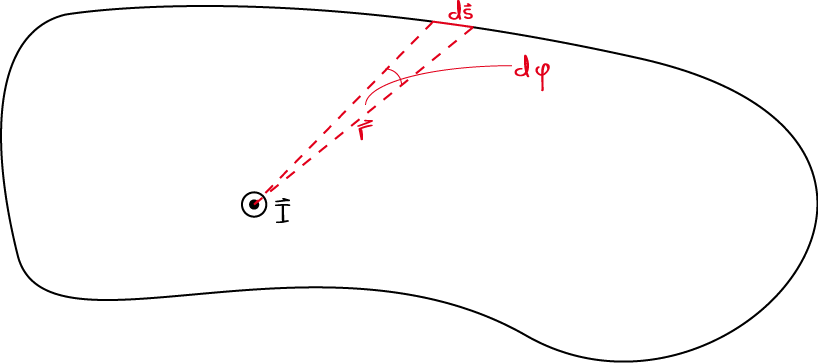
\includegraphics[width=0.4\linewidth]{skizzen/16/16_2B07}
\end{center}
\fbox{\parbox[c][][c]{0.33\textwidth}{\begin{align*} {\displaystyle \oint \vec{B} \cdot \vec{s} } & = \mu_0 \cdot I_{ges}\\ &= \mu_0 \cdot {\displaystyle \sum_{i=1}^{N} I_i } \end{align*}} }
\subsubsection{Ampere'sches Gesetz}
Für kontinuierliche Medien: $ I = {\displaystyle \int_A \vec{j}\cdot d\vec{A}} $\\
$$ \Rightarrow\underline{{\displaystyle\oint_C \vec{B}\cdot d\vec{s} = \mu_0\int_A \vec{j} \cdot d\vec{A}}} $$
A: von C umradnete Fläche\\
\break
Beispiel 1: Stromdurchflossener Leiter:
\begin{center}
	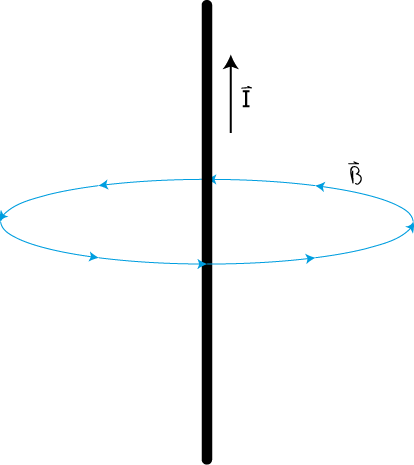
\includegraphics[width=0.4\linewidth]{skizzen/16/16_2B09}
\end{center}
\begin{itemize}
	\item $ |\vec{B}| $ hängt nur von Abstand $ r $ ab
	\item tangentiale Orientierung
\end{itemize}
\begin{math}
\mu_0 \cdot I = {\displaystyle\oint\vec{B}d\vec{s}} = B \cdot 2\pi r\\
\Rightarrow \underline{\underline{B(r) = \frac{\mu_0 \cdot I }{2\pi r}}}
\end{math}

\noindent Beispiel 2: Magnetfeld einer langen Spule:
\begin{center}
	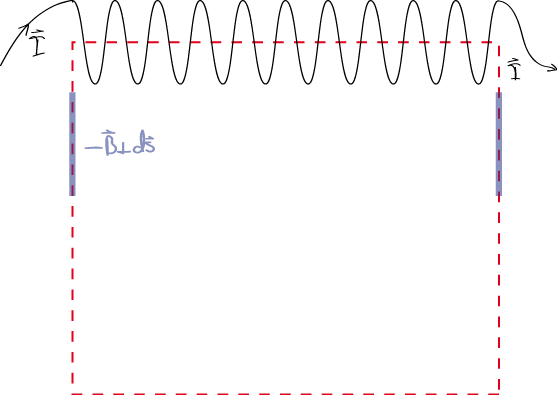
\includegraphics[width=0.6\linewidth]{skizzen/16/16_2B10}
\end{center}

\subsubsection{Das Ampere'sches Gesetz in differentieller Form}
Integralsatz von Stokes: $ {\displaystyle\oint\vec{B} \cdot d\vec{v} = \int_A (\nabla\times\vec{B} \cdot d \vec{A}) = \int_A rot\vec{B} \cdot d\vec{A}} $ \\
$ \Rightarrow {\displaystyle\oint\vec{B} \cdot d\vec{v} = \int_A (\nabla\times\vec{B}) \cdot\vec{A} = \mu_0 \cdot \int_A \vec{j} \cdot d\vec{A}} $
$$ \boxed{\Rightarrow \nabla\times\vec{B} = \mu_0 \cdot \vec{j}} $$
\begin{center}
	Ampere'sches Gesetz in differentieller Form
\end{center}

\subsubsection{Das Gesetz von Biot-Savart}
Suche Formulierung zur Berechnung des Beitrags $ d\vec{B} $ eines Leiterstückers von beliebig geformtem Leiter am Punkt P :
\begin{center}
	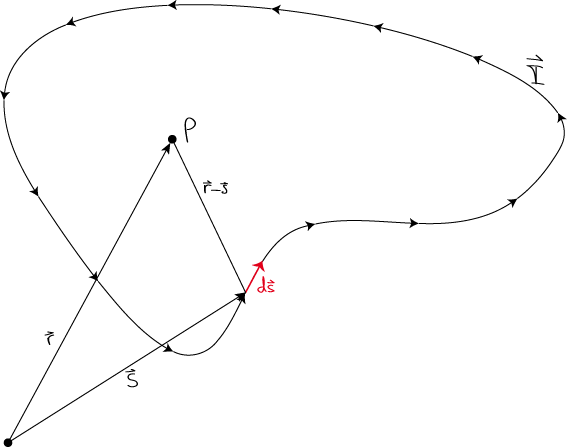
\includegraphics[width=0.4\linewidth]{skizzen/16/16_2B11}
\end{center}
$$ \boxed{d\vec{B} = \frac{\mu_0}{4\pi} \cdot I \cdot \frac{d\vec{s} \times (\vec{r}-\vec{s})}{|\vec{r}-\vec{s}|^3} } $$
($ \frac{1}{r^2} $ - Abstandsabhängigkeit)\\
genaue Herleitung komplex ($ \rightarrow $Theoretische Physik)\\
Gesamter Leiter: $ B(\vec{r}) = \frac{\mu_0 \cdot I}{4\pi} {\displaystyle\int_{Leiter}} \frac{d\vec{s} \times (\vec{r}-\vec{s})}{|\vec{r}-\vec{s}|^3} = \frac{\mu_0 \cdot I}{4\pi} {\displaystyle\int_{Leiter}} \frac{d\vec{s} \times \hat{e}_{\vec{r}-\vec{s}}}{|\vec{r}-\vec{s}|^2} $ \\
Zur Berechnung des Magnetfeldes beliebiger Stromverteilungen\\
(Vile Leiter: Addition der einzelnen Beträge)\\ \break
Beispiel: Magnetfeld eines elektrischen Ringstroms (entlang Symmetrieachse)
\begin{center}
	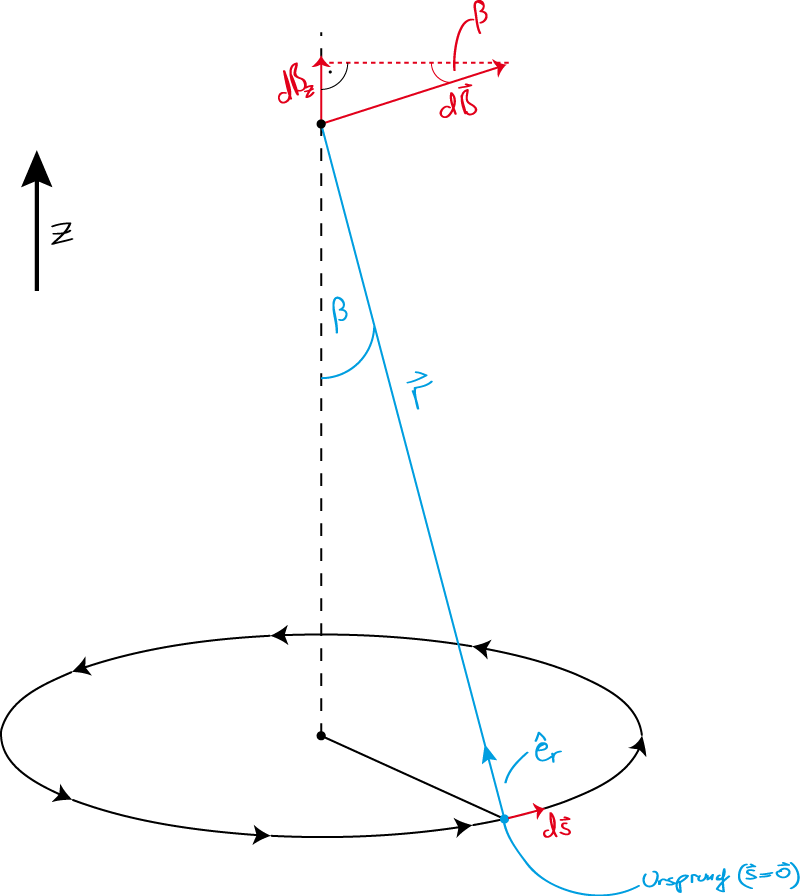
\includegraphics[width=0.6\linewidth]{skizzen/16/16_2B12}
\end{center}
\begin{align*}
	d\vec{B} &= \frac{\mu_0 \cdot I}{4\pi} \cdot \frac{d\vec{s} \times \hat{e}_r}{r^2} ;\hspace{1cm} d\vec{s} \perp \hat{e}_r\\
	&=\frac{\mu_0 \cdot I}{4\pi} \cdot \frac{ds}{r^2}
\end{align*}
Beachte: Beiträge in Ebene $ \perp z$ Kompensieren sich entlang der Symmetrieachse!
\begin{align*}
 dB_z &= dB\cdot \sin\beta = dB \cdot \frac{R}{r} = \frac{\mu_0 \cdot I}{4\pi} \cdot \frac{R}{r} \cdot \frac{1}{r^2} ds\\
 B_z &= \frac{\mu_0 \cdot I}{4\pi} {\displaystyle\oint_{Umfang}} \frac{R}{\underset{\text{konstant entlang Umfang}}{r^3}} ds = \frac{\mu_0 \cdot I}{4\pi} \cdot \frac{R}{r^3} {\displaystyle\oint}ds &&= \frac{\mu_0 \cdot I}{4\pi} \cdot \frac{R}{r^3} \cdot 2\pi R\\
 & &&=\frac{\mu_0 \cdot I}{2\pi} \cdot R^2\pi\frac{1}{(R^2+z^2)^{3/2}}\\
 & &&= \frac{\mu_0}{2\pi} \cdot \underbracket{\boxed{IR^2\pi}}_{\mu_{mg}} \cdot \frac{1}{(R^2+z^2)^{3/2}}\\
  && \Rightarrow B_z &=\underline{\underline{ \frac{\mu_0}{2\pi} \cdot \mu_{mg} \cdot r^{-3}}}
\end{align*}
Analogie: Elektrischer Dipol: $ E_r(\vec{r}) \sim \frac{\rho}{r^3} $\\
Helmholtz-Spulenpaar:
Mit einer Anordnung aus zwei kreisförmigen Spulen im Abstand von dem halben Durchmesser kann ein sehr homogenes Magnetfeld erzeugt werden. (Abweichung $ <1\% $ für $ z<0.3\cdot R $) \begin{center}
	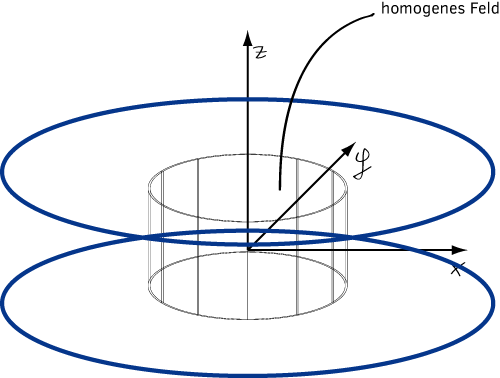
\includegraphics[width=0.5\linewidth]{skizzen/16/16_2B13}
\end{center}
$$ B_z (0,0,z) = \frac{\mu_0}{2}I\left( \frac{R^2}{(R^2+(z+\frac{R}{2})^2 )^{3/2} }+\frac{R^2}{(R^2+(z+\frac{R}{2})^2 )^{3/2} }\right)  $$
Entwicklung in eine Potenzreihe liefert näherungsweise $  B_z (0,0,z) = \frac{\mu_0 I}{(5R^2/4)^{3/2}}\left( 1-\frac{144z^4}{125R^4} \right)  $
\subsubsection{Zusammenhang zwischen elektrischen und magnetischen Feld}
\underline{Gedankenexperiment}: \\
2 Ladungen: \hspace{5mm} $ +q $ , $ -q $ ; Masse $ m $ , Geschwindigkeit $ \vec{v} $ \\
Bewegtes Koordinatensystem ($ \vec{v} $) ; Ladungen ruhen
\begin{center}
	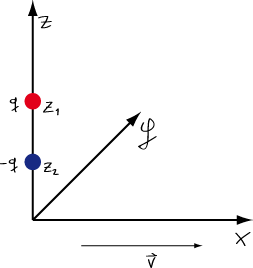
\includegraphics[width=0.4\linewidth]{skizzen/16/16_2B14}
\end{center}
Coulombkraft:
\begin{align*}
	m\ddot{z_1} &= - \frac{1}{4\pi\epsilon_0} \frac{q^2}{(z_1-z_2)^2} \\
	m\ddot{z_2} &= \frac{1}{4\pi\epsilon_0} \frac{q^2}{(z_2-z_1)^2}
\end{align*}
Ruhendes Koordinatensystem:
\begin{center}
	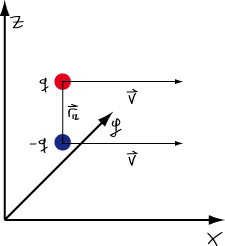
\includegraphics[width=0.4\linewidth]{skizzen/16/16_2B15}
\end{center}
zusätzlich: $ \vec{B} $-Feld
\begin{align*}
	\vec{B}(z_1) &= \frac{\mu_0}{4\pi}q\frac{\vec{r}_{12} \times \vec{v}}{| \vec{r}_{12} |^3} \hspace{5mm} \text{aus Biot-Savart} \\
	B_y(z_1) = \frac{\mu_0}{4\pi}qv\frac{1}{( z_1-z_2 )^2}
\end{align*}
Zusätzliche Lorentzkraft auf obere Ladung: \\
$$ \vec{F_l} = q \cdot (\vec{v}\times \vec{B}) $$
$$ |\vec{F_l}| = q \cdot v \cdot B_y = q^2 \cdot \frac{\mu_0}{4\pi} \cdot v^2 \cdot \frac{1}{(z_1-z_2)^2} $$
Gesamtkraft: $ F=F_L+F_C $
\begin{align*}
&-\frac{1}{4\pi\epsilon_0} \frac{q^2}{(z_1-z_2)^2} + \frac{\mu_0}{4\pi} \frac{q^2v^2}{(z_1-z_2)^2}\\
&-\frac{1}{4\pi\epsilon_0} \frac{q^2}{(z_1-z_2)^2} \underbrace{(1-\epsilon_0\mu_0v^2)}_{\text{kleinere Beschleunigung im ruhendem System!}}
\end{align*}

$ \epsilon_0 \cdot \mu_0 = c^{-2}$ ; $  \underbrace{c \approx \SI{2,998e8}{\meter\per\second}}_{\text{Lichtgeschwindigkeit im Vakuum}} = (\epsilon_0\mu_0)^{-1/2} $ \\
$ \Rightarrow $ Beschleunigung ist um $ \underbrace{( 1-\frac{v^2}{c^2} )}_{\text{aus \underline{Relativistischer Mechanik!}}} $ kleiner!\\
$ \Rightarrow $ In relativistischer Beschreibung laufen die beiden Experimente in beiden Bezugssystemen gleich ab! \\
$ \Rightarrow $ Transformation der physikalischen Größen beinhalten Umwandlung von elektrische in magnetische Kraft!